\documentclass{article}

\usepackage[letterpaper,margin=1in]{geometry}
\usepackage[skip=12pt]{parskip}

\usepackage{graphicx}
\usepackage{svg}
\usepackage{wrapfig}
\usepackage{subcaption}

\title{Lab 5 -- MPI Barnes-Hut}
\author{Jerry Reinoehl}
\date{CS380P Fall 2023}

\begin{document}
\maketitle{}

\section{Approach}
To implement the Barnes-Hut algorithm I first created a spatial partition tree
(quadtree) and particle data structure.
When a particle is inserted into the tree, the tree recursively divides
regions into four subregions such that there is never more than one particle in
the same subregion.
After all particles have been inserted into the tree, the center of mass of
each subregion is computed from the bottom node up.
Next, for each particle, the force applied to the particle can be calculated
by traversing the tree.
If the particle is far enough away from a region, determined by the length of
the region $l$, the distance to the region $d$, and the threshold $\theta$,
then the force on the particle from that region can be calculated with the
region's center of mass rather than each individual particle within the region,
thus saving many computations and time.
Finally, the calculated force is applied and the particle's position and
velocity is updated.

\begin{figure}[htbp]
  \centering
  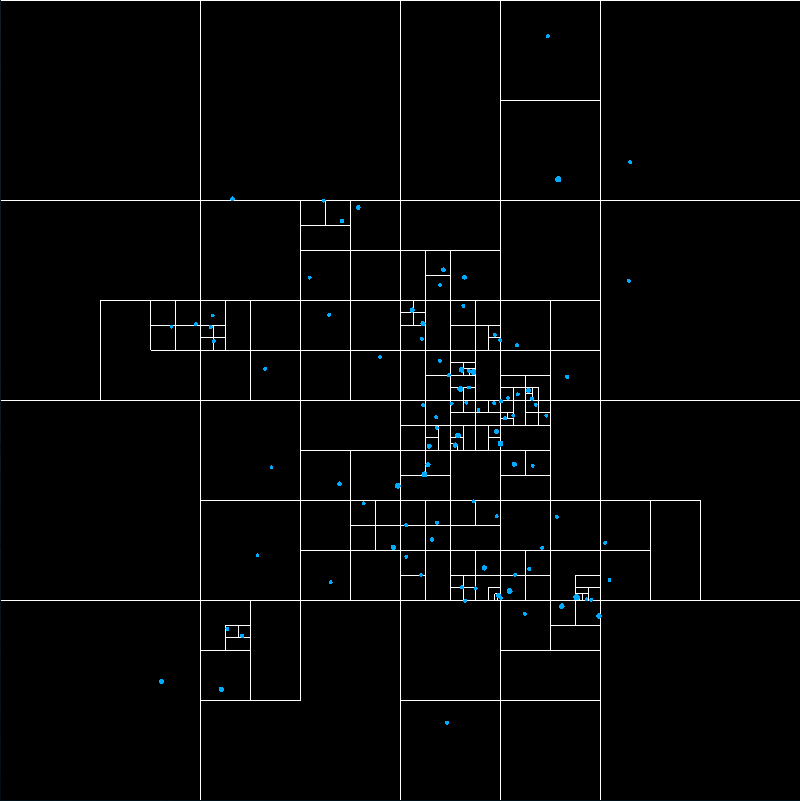
\includegraphics[scale=0.4]{tree.png}
  \caption{Visualization of Quadtree Space Partitioning}
\end{figure}

The graph below shows the amount of time spend in each phase of the sequential
computation for 100,000 particles with a threshold of 0.5: tree construction,
center of mass computation, and force calculation.
The majority of the computation time (93.49\%) comes from computing the force applied to
each particle by traversing the quadtree.
Therefore, this portion is the best candidate to parallelize with MPI to
achieve a speedup.

\begin{center}
  \includesvg[scale=1.0]{comptime.svg}
\end{center}

The first process (rank 0) reads in the particles from an input file.
It then will broadcast the num of particles read to all other processes with an
\texttt{MPI\_Bcast}.
All other processes will then allocate a buffer with enough space to hold the
given number of particles.
The first process will then broadcast the particles to the other processes.
Each process then constructs a quadtree with all of the particles and computes
the center of mass of each subregion.
However, for the force computation and particle updates, the particles are
evenly divided among the processes.
Each process will concurrently traverse their tree to compute and update their
set of particles.
After each process computes and applies the force to each of its particles it
will broadcast its set of particles with an \texttt{MPI\_Ibcast} to all other
processes and repeat.

\section{Performance}

In the graphs below we compare the average loop time as we change the number of
processes, the number of particles, and the threshold.
We can see that when there are few force computations, such as for 100
particles with a threshold of 1 or with just 10 particles, the sequential implementation beats the MPI
implementation.
We also notice that as we increase the number of processes the execution time
grows.
This is because the overhead of communication outweights the time spend doing
actual work.
However, as we increase the amount of work done per loop, such as by decreasing the
threshold or increasing the number of particles, we start to see some speedup.

\begin{center}
  \includegraphics[scale=0.48]{looptime10.png}
\end{center}

\begin{center}
  \includegraphics[scale=0.48]{looptime100.png}
\end{center}

We start to notice some speedup as we increase the number of particles to 100
and drop the threshold to 0.2.
We notice much better scaling as we increase the number of particles to
100,000.
The best speedup obtained was 3.55 for 100,000 particles with a threshold of
0.2 with 8 processes.
This indicates that the parallel MPI solution should really only be used when
simulating a large number of particles over many steps.
For the MPI solution to be effective the amount of work per loop should take
much more time than the broadcasting of particles between processes.
The speedup of the MPI implementation improves up to about 8 processes, the
number of cores on the test machine.

\begin{center}
  \includegraphics[scale=0.48]{looptime100000.png}
\end{center}

\section{OS and Hardware Details}

\begin{center}
\begin{tabular}{|l|l|}
  \hline
  \multicolumn{2}{|c|}{\bf OS Details} \\ \hline
  OS & Arch Linux        \\ \hline
  Kernel & 6.6.2-arch1-1 \\ \hline
  Architecture & x86\_64 \\ \hline
  Memory & 16 GiB        \\ \hline
  MPICH version & 4.1.2  \\ \hline
  GCC version & 13.2.1  \\ \hline
\end{tabular}
\end{center}

\begin{center}
\begin{tabular}{|l|l|}
  \hline
  \multicolumn{2}{|c|}{\bf CPU Hardware Details} \\ \hline
  Name & AMD Ryzen 7 PRO 4750U Processor \\ \hline
  Cores & 8                                   \\ \hline
  Threads & 16                                \\ \hline
  Clock rate & 1.7 GHz                        \\ \hline
  Cache L1 & 64 KiB (per core)                 \\ \hline
  Cache L2 & 512 MiB (per core)                \\ \hline
  Cache L3 & 8 MiB (shared)                    \\ \hline
\end{tabular}
\end{center}

\section{Time Spend on Lab}

\begin{center}
  \begin{tabular}{|l|c|}
    \hline
    \multicolumn{2}{|c|}{\bf Time Breakdown} \\ \hline
    Sequential Implementation & 10 hrs      \\ \hline
    OpenGL Visiualization     &  3 hrs      \\ \hline
    MPI Parallel Implementation & 9 hrs     \\ \hline
    Report & 8 hrs                          \\ \hline
    \bf{Total} & \bf{30 hrs}                \\ \hline
  \end{tabular}
\end{center}

\end{document}
